%%----------------------------------------------------------------------
%%----------------------------------------------------------------------
\clearpage
\pagetitle{Introduction}

\begin{columns}

  \emph{Legacies} is an unofficial skirmish campaign for Games
  Workshop's \emph{Warhammer 40,000}.  Its core is a set of eight
  thematic missions designed for \emph{Recon Squad}, an unofficial
  skirmish variant of \emph{40k} similar to Games Workshop's official
  \emph{Kill Team} rules.  In a Recon Squad game, players field small
  armies and all of their models act independently.  This makes for a
  very different \emph{40k} experience, focused on the heroics and
  sacrificies of everyday grunts and squad leaders.

  Those skirmish missions are woven into a campaign by a set of eight
  legacies.  Players choose one at the start of the campaign and
  strive to win specific missions to build that reputation.  At the
  end of the campaign comes the Cataclysm, in which all the recon
  squads and some reinforcements fight a final team battle while also
  trying to fulfill their legacy.

  % Following the events of \emph{The Debacle on Caldor IV} it has
  % become clear that the legendary \emph{Scythe of Unbound Light}
  % exists and is immeasurably important.  This discovery has spun the
  % maelstrom of conflict on Caldor IV to even dizzier velocities.
  % Unfortunately, the destruction of the planet is also now inevitable
  % with the Imperium having begun Exterminatus.  With every army
  % shattered and communication all but impossible, it is up to the
  % individual commanders and warriors in the field to rise to the
  % moment.  \emph{The Twilight of Caldor IV} plots the heroics of small
  % bands of warriors furiously moving into position to help their
  % alliance claim the relic before the end.

\columnbreak
\noindent\fbox{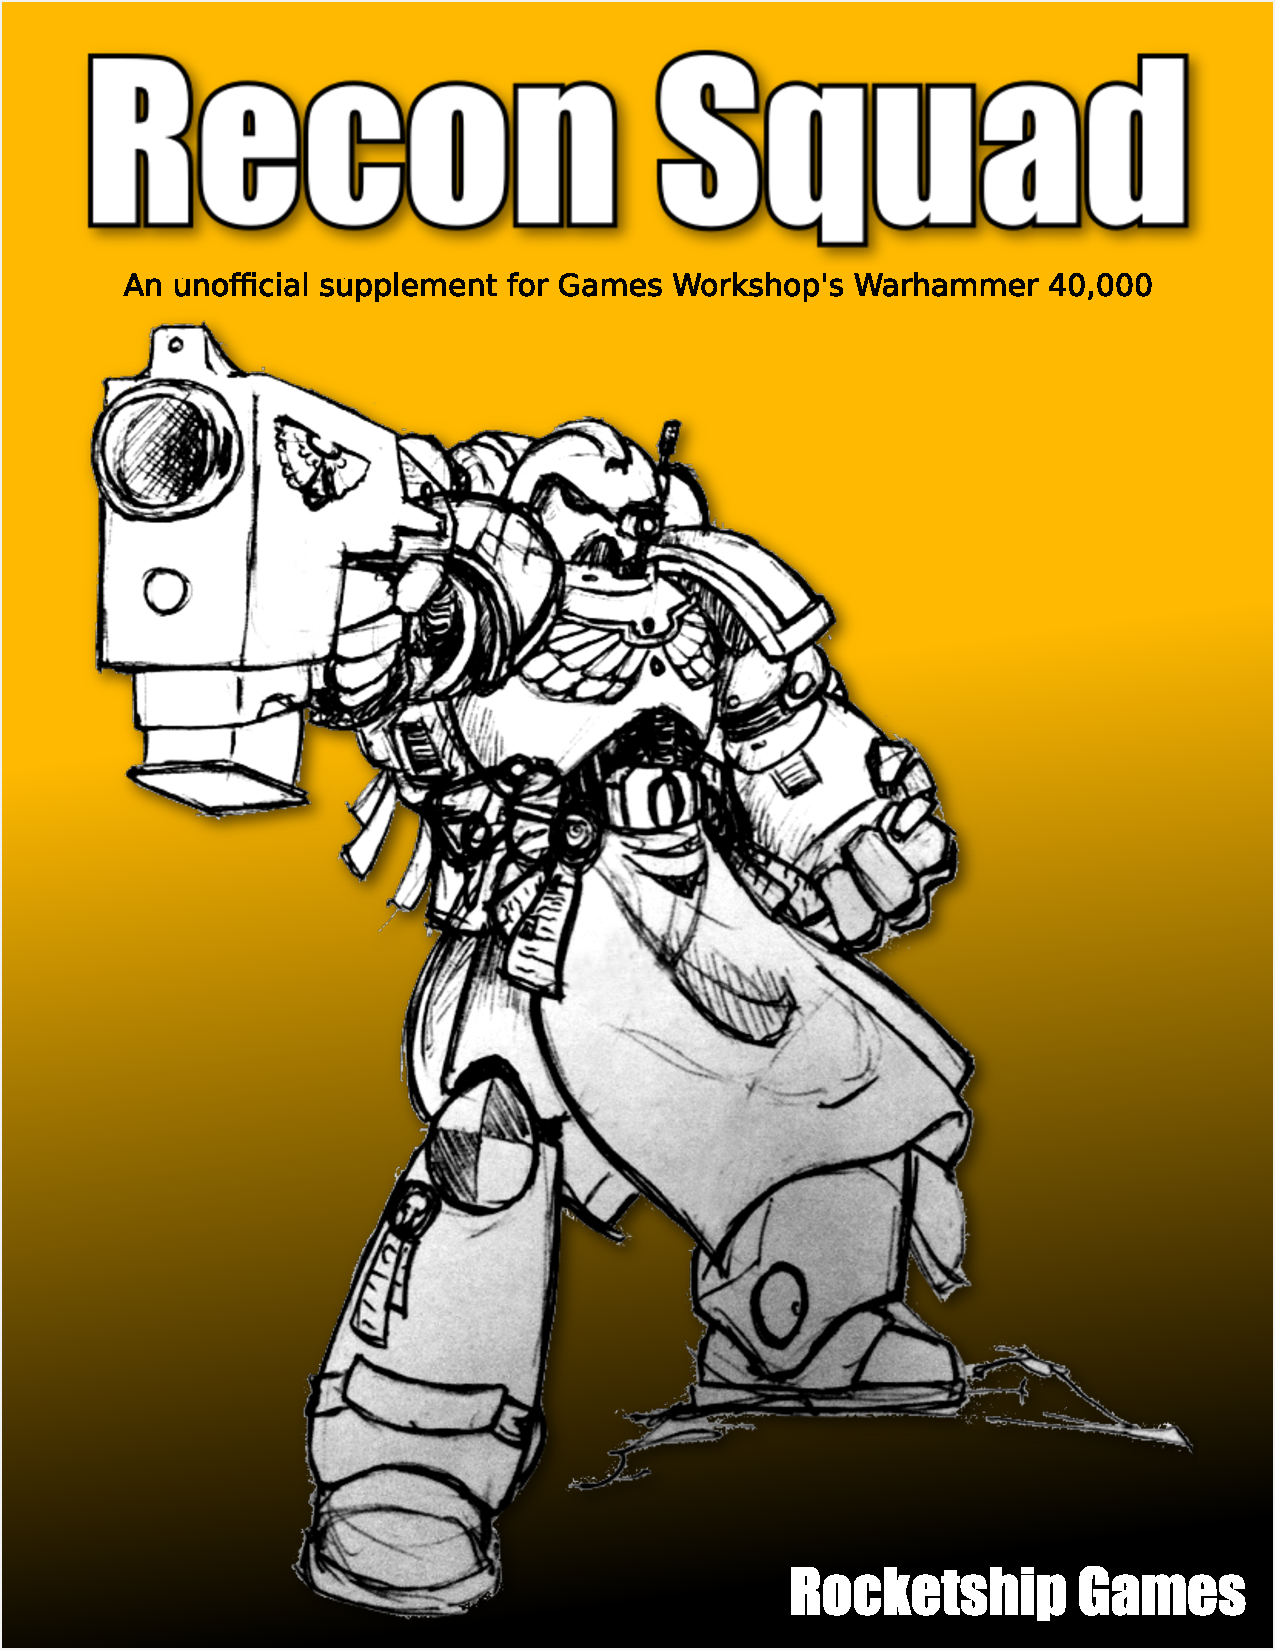
\includegraphics[width=\linewidth]{art/recon-squad.pdf}}

\missionheading{Overview}

\emph{The Twilight of Caldor IV} is played as four rounds of Recon
Squad skirmishes, each capturing a small but pivotal incident in the
closing chapters of the war.  Full rules for Recon Squad are available
here:

\centerline{\url{rocketshipgames.com/games/recon-squad/}}

\smallskip%
Each squad is working toward a particular legacy inside the grand
history of the greater conflict:

\begin{squishitemize}
\item \textbf{Bodyguards:} Fierce defenders of critical battlefield
  leaders and personnel;

\item \textbf{Excavators:} Daring explorers, technical experts, and
  artifact raiders \emph{par excellence};

\item \textbf{Headhunters:} Precision instruments of assassination and
  targeted violence;

\item \textbf{Killers:} Shattered fighters disconnected from anything
  but maniacal bloodshed;

\item \textbf{Penetrators:} Sharpened blades able to break through any
  armor or defense;

\item \textbf{Scouts:} Reckless adventurers dancing in the jaws of
  death for more information;

\item \textbf{Sentinels:} Implacable defenders and masters of
  impromptu fortification building;

\item \textbf{Warriors:} Hardened veterans that have been through
  everything and haven't seen the end.
\end{squishitemize}

%\begin{sidestory}{2cm}{Thought for the Day}
%\end{sidestory}


Their path toward those legacies is defined by the missions they
tackle, as attackers or defenders:

\smallskip\centerline{\begin{tabular}{C{1.25in}C{1.25in}}
\textbf{Ambush} & \textbf{Encirclement}\\
\textbf{Assassination} & \textbf{Excavation}\\
\textbf{Battlefield} & \textbf{Installation}\\
\textbf{Breakthrough} & \textbf{Skirmish}\\
\end{tabular}}

\smallskip%
Successes and failures at those challenges will define both the
squad's place in history, and their alliance's ability to secure
\emph{The Scythe}.

\missionheading{Setup}

For each alliance, print and cut apart enough sets of the~8 legacy
cards at the end of this section to have at least one card per player.
The players in each alliance then choose cards together, one per
player.  Note that this is a choice, not a random pull.  No card type
may be selected twice within an alliance unless all types have been
chosen at least once.

\missionheading{Legacies}

Each legacy has three Twilight missions, a Cataclysm objective, and a
legacy bonus.  To achieve their legacy, players must accomplish the
Cataclysm objective in that battle of the next campaign component.  If
they win at least two of the three Twilight missions in the given role
of attacker, defender, or either then they will receive their legacy
bonus in The Cataclysm.

Players' legacy cards, their results, and whether or not they
succeeded at their Twilight missions are all public knowledge
throughout the campaign.

\end{columns}

%%----------------------------------------------------------------------
%%----------------------------------------------------------------------
\vfill
\noindent
\begin{minipage}[t]{1.0\linewidth}\centering%
\rowcolors{2}{gray!12}{white}\setlength{\tabcolsep}{3pt}%
\resizebox{\linewidth}{!}{\begin{tabular}{|l|C{1in}|C{1in}|C{1in}|C{1in}|C{1in}|C{1in}|C{1in}|C{1in}|}
\hline
\rowcolor{gray!25} {\bf Mission}       
                    & {\bf Bodyguards}  & {\bf Excavators}& {\bf Headhunters}   & {\bf Killers}   & {\bf Penetrators}&{\bf Scouts}   & {\bf Sentinels} & {\bf Warriors}\\
\hline
\hline
{\bf Ambush}        & Defender          & Either         & Attacker             &                 &                 & Attacker       &                 &               \\
{\bf Assassination} & Defender          &                & Attacker             &                 & Attacker        &                &                 &               \\
{\bf Battlefield}   &                   &                &                      & Either          &                 &                &                 & Either        \\
{\bf Breakthrough}  & Attacker          &                &                      &                 & Attacker        &                & Defender        &               \\
{\bf Encirclement}  &                   &                &                      & Attacker        &                 &                & Defender        & Defender      \\
{\bf Excavation}    &                   & Either         & Either               &                 &                 & Either         &                 &               \\
{\bf Installation}  &                   & Either         &                      &                 & Attacker        &                & Defender        &               \\
{\bf Skirmish}      &                   &                &                      & Either          &                 & Either         &                 & Either        \\
\hline
\end{tabular}}

\small\it\smallskip
Twilight mission and role requirements for the legacies.
\end{minipage}
\vfill

\vbox to 0pt{}

%%----------------------------------------------------------------------
%%----------------------------------------------------------------------
\clearpage

\begin{columns}

\missionheading{Round Pairings}

Players are paired with an opponent for each match from another
alliance as best as possible given the number of players.  Teammates
should only battle if no other set of pairings is possible.  In that
rare case, their alliance earns the lesser of the two players' victory
points.  The players though each claim their respective victory points
toward the individual rankings as well as credit toward their Twilight
missions.

Before each round the alliances alternate nominating a player,
mission, and role (attacker or defender).  For the first round the
alliances alternate in order of total victory points from the end of
\emph{The Debacle}, but those victory points are not actually carried
forward into this campaign component.  In the second and third rounds
the alliances alternate in order by total accumulated victory points.

The opposing alliance with the most unmatched players in the same
win/loss/draw bracket as the nominated player then responds with an
opponent and a table for the match.  If the opposing alliances have an
equal number of unmatched players in the bracket then one alliance is
randomly selected to respond.  The opponent must be chosen from that
alliance's unmatched players in the same win/loss/draw bracket as the
nominated player.  If there are no such players then the opponent must
be chosen from the closest possible win/loss/draw bracket.  No two
players may ever be matched more than once.

Alliances can nominate any players, missions, and roles they like.
However, they should use those nominations to ensure their players get
chances to complete the Twilight missions for their legacy.

Players should use the checkboxes on their legacy cards to record
victories toward the Twilight mission requirements.  It does not
matter if the player was nominated or the responding opponent.  They
simply have to win that mission in that role at some point in this
campaign component.  Similarly, a player can attempt a mission and
role pair multiple times.  However, they gain nothing by winning the
same mission and role pair multiple times.

\end{columns}


%%----------------------------------------------------------------------
%%----------------------------------------------------------------------
\clearpage
\pagetitle{The Twilight: Mission Pack}


All of the missions are played on a~4'x4' table.

The variable game length rule is used in all missions unless noted otherwise.

  Roll a~D6 before any
deployment.  Night Fighting is in effect for Turn~1 on a~4+; on a~1
or~2 it takes effect on Turn~5 and thereafter.

The winner of a~D6 roll off decides to deploy first or second.  After
both players deploy, the player that deployed first chooses to play
first or second.  The player to go second may attempt to Seize the
Initiative.


A major victory is worth 10 points to the winner and 0 to the loser.
Victory is 7 and 3
Draw is 5 and 5

Plus the two bonus points.

Better victories trump others, e.g., meeting the conditions for a
major victory trumps the conditions for a minor victory.

Missions to be specified in more detail...

\missionheading{Ambush}

The Defender is given an AV10/10/10 HP2 truck with 5 embarked NPCs
with sub-Guardsman stats.  The truck takes dangerous terrain tests on
a 2+ and always takes a dangerous terrain test if it moves flat out.
The truck starts at one end of the board and it or the NPCs must make
it to the far edge.  The Attacker Outflanks.


\missionheading{Assassination}

An NPC with Guardsman-ish stats is placed in control of the Defender,
who loses if it dies.


\missionheading{Battlefield}

Kill points with Dawn of War setup.


\missionheading{Breakthrough}

Attacker has to break into the defender's deployment zone.


\missionheading{Encirclement}

Kill points with the defender starting at the center of the table and
the attacker all around.


\missionheading{Excavation}

Similar to the scouring, several objectives of randomized value are
randomly placed inside a square at table center.  The defender starts
deployed in that square, the attacker is around the edges.


\missionheading{Installation}

A single objective is put forward slightly from the defenders leading
edge, inside an AV11 HP3 Small building.  The defender wins if they
hold that objective.  Otherwise the attacker wins.


\missionheading{Skirmish}

The basic mission from the Recon Squad packet: Vanguard and three objectives.
